\section{Struktura UML}

%% Z čeho se skládá, roztřídění jednotlivých diagramů

%%%%%%%%%%%%%%%%%%%%%%%%%%%%%%%%%%%%%%%%%%%%%%%%%%%%%%%%%%%%%%%%%%%%%%%%
%% Slide

\begin{frame}{Struktura UML}

\begin{figure}
	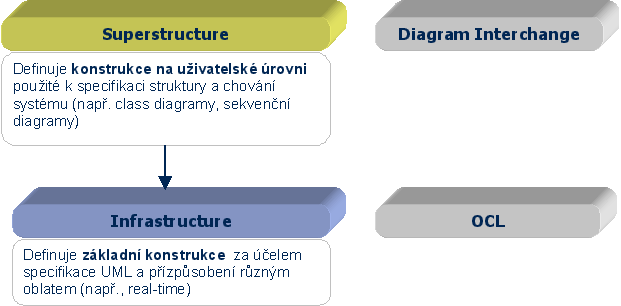
\includegraphics[width=80mm]{img/standard_uml.png}
	\caption{UML 2.0}
\end{figure}
	
\end{frame}

%%%%%%%%%%%%%%%%%%%%%%%%%%%%%%%%%%%%%%%%%%%%%%%%%%%%%%%%%%%%%%%%%%%%%%%%
%% Slide

\begin{frame}{Standard UML}

\onslide<+-> Standard UML 2.x má 4 hlavní části
\begin{itemize}
	\item<+-> Superstructure
	\onslide<+->
	\begin{itemize}
		\item Popisuje diagramy a jejich prvky
	\end{itemize}	
	
	\item<+-> Infrastructure
	\onslide<+->
	\begin{itemize}
		\item Metamodel na kterém založena Superstructure
		\item Meta-Object Facility (MOF)
		\begin{itemize}
			\item Metamodelovací architektura
			\item 4 vrstvy
		\end{itemize}

	\end{itemize}

	\item<+-> Object Constraint Language (OCL)
	\onslide<+->
	\begin{itemize}
		\item Pravidla pro prvky modelů
		\item Vstupní, výstupní podmínky, invarianty
		\item Možno použít pro formální specifikaci programu
		\item Komplikované, používá se mixovaná syntaxe
	\end{itemize}

	\item<+-> Diagram Interchange
	\onslide<+->
	\begin{itemize}
		\item Definice XML struktur pro výměnu modelů mezi nástroji
		\item Pro výměnu metadat metamodelů je XMI
	\end{itemize}

\end{itemize}
	
\end{frame}

%%%%%%%%%%%%%%%%%%%%%%%%%%%%%%%%%%%%%%%%%%%%%%%%%%%%%%%%%%%%%%%%%%%%%%%%
%% Slide

\begin{frame}{Základní pojmy}

\onslide<1-> Tři základní stavební bloky UML modelu

\begin{itemize}
	\onslide<2->
	\item Předměty
	
	\onslide<5->
	\begin{itemize}
		\item Structural Things
		\item Behavioural things
		\item Grouping Things
		\item Annotational Things
	\end{itemize}
	
	\onslide<3->
	\item Relace
	\onslide<6->
	\begin{itemize}
		\item Vztahy mezi předměty
		\item Různé druhy
	\end{itemize}
	
	\onslide<4->
	\item Diagramy
	\onslide<7->
	\begin{itemize}
		\item Zachycují různé pohledy na modelovaný systém
		\item 13 typů (současný standard dokonce 14)
	\end{itemize}
\end{itemize}

\end{frame}

%%%%%%%%%%%%%%%%%%%%%%%%%%%%%%%%%%%%%%%%%%%%%%%%%%%%%%%%%%%%%%%%%%%%%%%%
%% Slide

\begin{frame}{Základní pojmy II}


\onslide<1-> Pravidla řídící tvorbu modelu

\begin{itemize}
	\onslide<2->
	\item Specifikace (Specification)
	\onslide<6->
	\begin{itemize}
		\item Sémantický základ
	\end{itemize}
	
	\onslide<3->
	\item Podrobnosti (Adornments)
	\onslide<7->
	\begin{itemize}
		\item Stejný element na různých diagramech s různou mírou detailů
	\end{itemize}
	
	\onslide<4->
	\item Obecná dělení (Common Divisions)
	\onslide<8->
	\begin{itemize}
		\item Klasifikátor a instance
		\item Rozhraní a implementace
	\end{itemize}
	
	\onslide<5->
	\item Mechanismy rozšíření
	\onslide<9->
	\begin{itemize}
		\item Stereotypy
		\begin{itemize}
			\item Např. $<<$interface$>>$
		\end{itemize}
		\item Omezení (Constraints)
		\begin{itemize}
			\item Object Constraint Language (OCL)
		\end{itemize}
		\item Označené hodnoty (Tagged Values)
	\end{itemize}
\end{itemize}
	
\end{frame}

%%%%%%%%%%%%%%%%%%%%%%%%%%%%%%%%%%%%%%%%%%%%%%%%%%%%%%%%%%%%%%%%%%%%%%%%
%% Slide

\begin{frame}{Typy relací}

\onslide<+-> Základní typy vztahů jsou
\bigskip

\begin{columns}[T]

	\begin{column}{0.5\textwidth}
		\begin{itemize}
			\item<+-> Asociace
			\onslide<+->
			\begin{itemize}
				\item Obecná souvislost předmětů
			\end{itemize}
			\item<+-> Závislost
			\item<+-> Generalizace
			\item<+-> Realizace
		\end{itemize}
	\end{column}

	\begin{column}{0.5\textwidth}
		\begin{flushleft}
		\onslide<1->
		\begin{figure}
			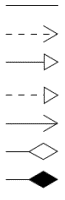
\includegraphics[width=10mm]{img/relace/relace.png}
			\caption{Typy relací}
		\end{figure}
		\end{flushleft}
	\end{column}

\end{columns}	

\end{frame}

%%%%%%%%%%%%%%%%%%%%%%%%%%%%%%%%%%%%%%%%%%%%%%%%%%%%%%%%%%%%%%%%%%%%%%%%
%% Slide

\begin{frame}{Druhy diagramů}


	
\end{frame}

%~ \begin{itemize}
%~ 
%~ \end{itemize}
